% Geometry for page layout
\documentclass[10pt]{article}
\usepackage[utf8]{inputenc}
\usepackage[T1]{fontenc}
\usepackage[english]{babel} % Language 'english' or 'frenchb', delete out/ if changing language
\usepackage{geometry}
\geometry{a4paper, margin=1in}

% Packages
\usepackage{amsmath}
\usepackage{graphicx}
\usepackage{subcaption}
\usepackage{fancyhdr}
\usepackage{lipsum}
\usepackage{hyperref}
\usepackage{microtype}
\usepackage{multicol}
\usepackage{csquotes}
\usepackage{listings}
\usepackage{xcolor}
\usepackage{sectsty}
\usepackage{enumitem}
\usepackage{array}
\usepackage{booktabs}
\usepackage{pdfpages}
\usepackage{pdfx}
\usepackage{indentfirst}
\usepackage{parskip}
\usepackage[scaled]{helvet}
\renewcommand{\familydefault}{\sfdefault}
\setlength{\parindent}{15pt}
\setlength{\parskip}{1em}

% Definitions
\definecolor{bleu_ece}{HTML}{00727A}
\newcommand{\bleuece}{bleu_ece}

\newcommand{\mytitle}{Internship Report Engineering Cycle, 2\textsuperscript{nd} year 2023/2024}
\newcommand{\myauthor}{Pierre LAPOLLA}

% Hyperref setup
\hypersetup{
    colorlinks=true,
    linkcolor=\bleuece,
    urlcolor=black,
    citecolor=black,
    pdfborder={0 0 0}
}

% Section styles
\sectionfont{\color{\bleuece}}
\subsectionfont{\color{\bleuece}}
\subsubsectionfont{\color{\bleuece}}


% Header and footer
\fancypagestyle{plain}{
    \fancyhf{}
    \fancyhead[L]{}
    \fancyhead[C]{}
    \fancyhead[R]{\vspace{-2em}
\includegraphics[height=5em]{images/logo_ece}}
    \fancyfoot[L]{\scriptsize \textit{\mytitle}}
    \fancyfoot[C]{\thepage}
    \fancyfoot[R]{\scriptsize \textit{\myauthor}}
    \renewcommand{\headrulewidth}{0pt}
    \renewcommand{\footrulewidth}{0pt}
}
\pagestyle{plain}

% Title and authors, see text definition above
\title{\mytitle}
\author{\myauthor}
\date{}

\begin{document}
    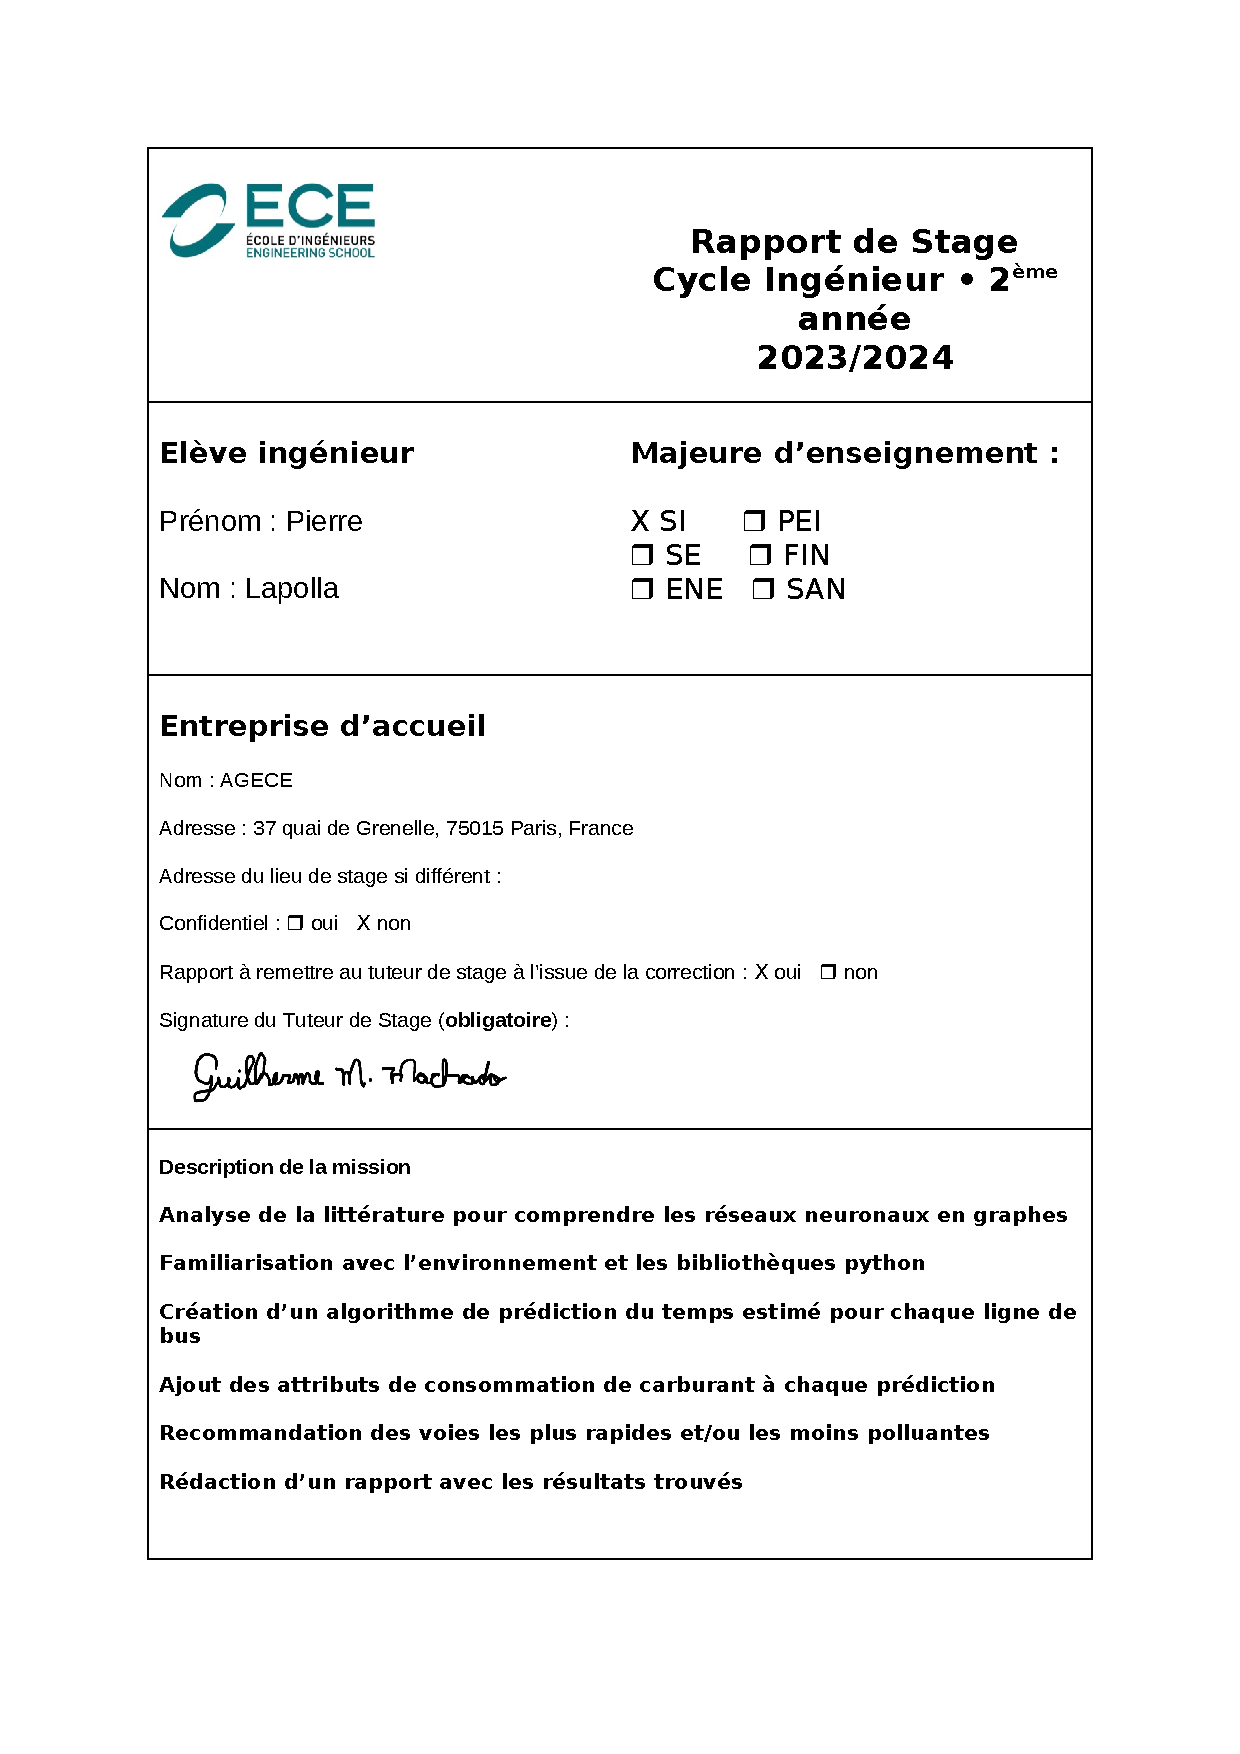
\includepdf{pdfs/cover.pdf}

    \maketitle
\tableofcontents


\section*{Acknowledgements}\label{sec:acknowledgements}
I would like to express my deepest gratitude to my mentors, Guilherme MEDEIROS MACHADO and Frédéric RAVAUT, for their
guidance and support throughout this internship.
The moments of exchange in meetings and the technical discussions were very enriching.
I would also like to thank the LyRIDS laboratory at ECE Paris for giving me with the opportunity to work on this project.
Finally, I would like to thank my colleagues for their feedback and assistance during this internship.

\vfill
\begin{center}
    \textit{The source code of this document is available at:
    \url{https://github.com/PierreLapolla/research_internship_report.git}}

    \textit{The \LaTeX{} template utilized for this document is available at:
    \url{https://github.com/PierreLapolla/tex_template.git}}
\end{center}
\newpage


    \section{Presentation of the Mission}\label{sec:presentation-of-the-mission}
    \subsection{Introduction}\label{subsec:introduction}
\textcolor{gray}
{Sets the stage for the mission, providing context and significance without going into specific project details.}

The primary purpose of my internship was to undertake a research project and produce a research paper on the assigned
topic.
The internship took place in a research laboratory associated with my engineering school, where I, along with
nine other students, was given a unique research topic.
Although the internship was positioned within an academic setting, the primary objective appeared to be more focused on
allowing us to independently explore and develop our research skills rather than contributing directly to the
laboratory's broader research goals.
This experience served as an opportunity for us to gain a deeper understanding of the research process, develop critical
thinking, and enhance our ability to work autonomously.

\subsection{Company Description}\label{subsec:company-description}
\textcolor{gray}
{Focuses on the company as a whole, giving background information and context that is broader than your specific
internship. Narrows down to the specific department,
    explaining its role within the company and setting up the context for your specific tasks.}


ECE Paris is a well-established engineering school, founded in 1919, with a long-standing tradition of excellence in
science and technology education.
The school is committed to producing well-rounded engineers equipped with the skills necessary for innovation,
international collaboration, and entrepreneurship.

Within this academic environment, Lyrids serves as the dedicated research laboratory of ECE Paris.
Established to promote high-level research, Lyrids focuses on several key areas including artificial intelligence, data
science,
cybersecurity, and connected systems.
The laboratory is organized into specialized research groups, each contributing to the advancement of knowledge in their
respective fields.
Lyrids plays a crucial role in integrating research into the academic curriculum, allowing students to engage with
cutting-edge projects and develop their research skills in a practical, hands-on environment.

\subsection{Purpose of the Internship}\label{subsec:purpose-of-the-internship}
\textcolor{gray}
{Details the objectives and goals specific to your internship experience, linking it to the company's broader mission.}

The primary objective of my internship was to propose a viable solution to the problem posed by my research topic.
This experience was designed not only to challenge me intellectually but also to foster my ability to work autonomously.
Throughout the internship, I gained significant hands-on experience, particularly in coding with \LaTeX{}, conducting
in-depth literature reviews, and strengthening my skills in neural network training and Python programming.

My expectation was to delve deeper into the field of artificial intelligence, and this internship fully met that goal.
The opportunity to focus on AI allowed me to explore and develop expertise in a domain that is not only fascinating but
also pivotal for my future career aspirations.
By engaging in research, I was able to acquire and refine a set of skills that will be highly beneficial as I continue
to pursue a career in engineering and technology.

\subsection{Context of the Internship}\label{subsec:context-of-the-internship}
\textcolor{gray}
{Describes the environment and any notable circumstances that influenced your internship, distinct from the daily tasks
and projects.}

The internship took place in a collaborative environment, with all ten interns working together in a classroom at the
school, conveniently located near the laboratory office.
This setup allowed for easy access to our mentors whenever guidance was needed.
While we didn't have access to many specialized resources, we made extensive use of Google Scholar and a specific
website that provides research papers, to which the school had a subscription.

The internship began with a loosely defined research topic, which required us to refine and narrow our focus as we
progressed.
Regular meetings with my mentor and another faculty member were crucial in planning and directing my research,
especially as the initial topic evolved significantly over time.
My mentor was supportive, particularly when I encountered challenges, and the collaborative atmosphere among the interns
in the shared space was a great advantage.
We frequently assisted each other, which enhanced the overall learning experience.

Working fully on-site was particularly beneficial for me, as I find it difficult to maintain focus when working from
home.
The structured environment of the school helped me stay productive and engaged with my work.

\subsection{Role and Responsibilities}\label{subsec:role-and-responsibilities}
\textcolor{gray}
{Specifically outlines what you did on a day-to-day basis, your tasks, and your contributions.}
During my internship, my responsibilities were structured into several key stages, each aimed at developing my research
project comprehensively.
The first stage involved conducting a thorough literature review, where I read various research papers to gain a deeper
understanding of the topic and familiarize myself with the relevant coding environment,particularly Python and its
associated packages.

Following the literature review, I moved on to the development stage, where my primary task was to propose and develop a
new solution to the problem presented by my research topic.
This phase required a combination of critical thinking,coding, and experimentation to arrive at a feasible solution.

The final major task was to document my work by writing a research paper detailing the problem, the methodology I
employed, the solution I developed, and the results of my work.
This paper was a significant deliverable, and after submitting it before the end of the internship, I received feedback
for revisions, which I am currently implementing.

In addition to these stages, I participated in a midterm presentation where I, along with the other interns, presented
our progress to the mentors.
This presentation served as a checkpoint, allowing us to receive constructive feedback and refine our approach as
needed.

Throughout the internship, all tasks and responsibilities were carried out individually, though we benefited from a
collaborative environment where we could assist each other.
While there were no specific performance goals to meet, the focus was on contributing to research, where even negative
or unexpected results were valuable.




    \section{Project Specifications and Schedule}\label{sec:project-specifications-and-schedule}
    \subsection{Project Overview}\label{subsec:project-overview}
The focus of my research project was on developing a model for multi-modal traffic prediction, specifically targeting
cars and wheelchairs.
This project aimed to address the unique challenges faced by mobility-impaired individuals,particularly those using
wheelchairs, by providing traffic predictions that consider their specific needs.
While existing platforms like Google Maps and Apple Maps offer itinerary recommendations, they often fall short when it
comes to detailed traffic prediction for wheelchair users.
Additionally, concerns over data privacy with these large platforms underscore the need for an open-source alternative.

The importance of this project lies in its potential to fill a gap in current traffic prediction systems by including
modes of transportation that are often overlooked, such as wheelchairs.
Unlike traditional itinerary recommendation systems, this project focuses on predicting traffic patterns rather than
merely suggesting routes, which adds an extra
layer of complexity and utility.

To tackle this problem, the project involved adapting the Diffusion Convolutional Recurrent Neural Network (DCRNN) model
to handle the complexities of multi-modal traffic prediction.
The model was enhanced to consider both cars and wheelchairs, with a specific focus on capturing the spatial and
temporal dependencies inherent in traffic data.
Additionally, a method was developed to derive wheelchair traffic data from the METR-LA dataset, which traditionally
contains only car traffic data.

The ultimate goal of the project was to produce a model capable of delivering accurate traffic predictions for both cars
and wheelchairs, thereby contributing to a more inclusive and comprehensive traffic prediction system.

\subsection{Objectives and Goals}\label{subsec:objectives-and-goals}
The primary goal of this project was to develop a model capable of performing accurate multi-modal traffic predictions
for both cars and wheelchairs.
While there were no strict performance targets set for the model, the project aimed to achieve a level of accuracy that
would be competitive with existing models in the field.
To evaluate the model's performance, we used Mean Absolute Error (MAE) and Root Mean Square Error (RMSE) as loss
metrics, comparing these results against those of other established models.

In addition to the technical objectives, I also had several personal goals for this project.
These included deepening my understanding of the research process and methodology, expanding my knowledge of machine
learning, and improving my skills in Python programming and LaTeX for academic writing.
These personal objectives were crucial for my professional development and aligned with my broader career aspirations in
the field of artificial intelligence and research.

\subsection{Scope of Work}\label{subsec:scope-of-work}
The development of the multi-modal traffic prediction model involved several key tasks and activities.
The first step was obtaining and understanding the METR-LA dataset, which provided the foundational data for car
traffic.
Given the absence of publicly available datasets for wheelchair traffic, a significant portion of the project involved
developing a method to derive wheelchair data from the existing car traffic data.

The next phase was designing a new architecture for the model, which required considerable effort in debugging and
refining the model to ensure it could effectively handle the complexities of multi-modal traffic prediction.
Training the model was another crucial task, which I accomplished using Kaggle's computational resources.
Although these resources were somewhat limited for working with Graph Neural Networks, they were sufficient to complete
the project.

The main deliverables of the project include the research paper, which thoroughly documents the methodology, data
derivation process, model architecture, and results.
Additionally, the newly created dataset, which integrates car and wheelchair traffic data, is another important output
of the project.
While the model itself was not saved due to its suboptimal performance, the insights and methodologies developed during
the project remain valuable contributions.

\subsection{Methodology and Approach}\label{subsec:methodology-and-approach}

\subsubsection{Overall Approach and Strategy}\label{subsubsec:overall-approach-and-strategy}
The project aimed to adapt an existing model, the Diffusion Convolutional Recurrent Neural Network (DCRNN), to handle
the complexities of multi-modal traffic prediction, specifically for cars and wheelchairs.
The overall approach involved several key stages: understanding and processing the existing METR-LA dataset, deriving
wheelchair traffic data,adapting the model architecture to accommodate multiple modes of transportation, and training
the model to predict traffic patterns.

\subsubsection{Key Methods and Techniques}\label{subsubsec:key-methods-and-techniques}
\begin{enumerate}
    \item \textbf{Model Adaptation}:
    \begin{itemize}
        \item
        The DCRNN model was adapted to consider both cars and wheelchairs by introducing a custom diffusion convolution
        operation to capture spatial dependencies in traffic data.
        Temporal dependencies were managed using Gated Recurrent Units (GRU), modified with the custom diffusion
        convolution to create a Diffusion Convolution Gated Recurrent Unit (DCGRU).
        \item
        The model's architecture retained the original encoder-decoder structure of the DCRNN but included key
        modifications.
        A new convolution operation, inherited from the PyTorch Geometric library's MessagePassing class,was used to
        enhance spatial dependency capture.
        Additionally, a multi-headed attention mechanism was added to allow the model to differentiate between the
        various locomotion modes.
    \end{itemize}

    \item \textbf{Data Derivation}:
    \begin{itemize}
        \item
        Due to the lack of available wheelchair traffic data, a novel method was developed to derive this data from the
        car traffic data in the METR-LA dataset.
        The process involved calculating an accessibility score using OpenStreetMap data, which was then applied to
        adjust the car traffic speeds to reflect wheelchair speeds.
        The final wheelchair traffic data was generated by scaling and introducing noise to simulate real-world
        variability.
    \end{itemize}

    \item \textbf{Training and Evaluation}:
    \begin{itemize}
        \item
        The model was implemented using PyTorch and associated libraries, with training conducted on the Kaggle
        platform.
        The dataset was split into training, validation, and test sets, with inputs shaped to capture various features,
        including speed, time of day, day of the week, and locomotion mode.
        \item
        Model performance was evaluated using Mean Absolute Error (MAE) and Root Mean Square Error (RMSE)
        metrics,comparing results against baseline models.
        The evaluation revealed that while the model performed well for individual modes (cars or wheelchairs), its
        performance on combined multi-modal predictions was less satisfactory, highlighting the complexity of the task.
    \end{itemize}
\end{enumerate}

\subsubsection{Challenges and Solutions}\label{subsubsec:challenges-and-solutions}
One of the main challenges was the derivation of wheelchair traffic data, as no pre-existing datasets were available.
The innovative method developed to generate this data introduced potential biases, but it was a necessary step given the
data constraints.
Another challenge was the model's scalability and generalization, as its performance varied significantly across
different transportation modes.
While the model showed promise, further improvements in architecture and data collection are necessary for better
scalability and generalization.

\subsection{Project Timeline}\label{subsec:project-timeline}
\begin{figure*}[htbp]
    \centering
    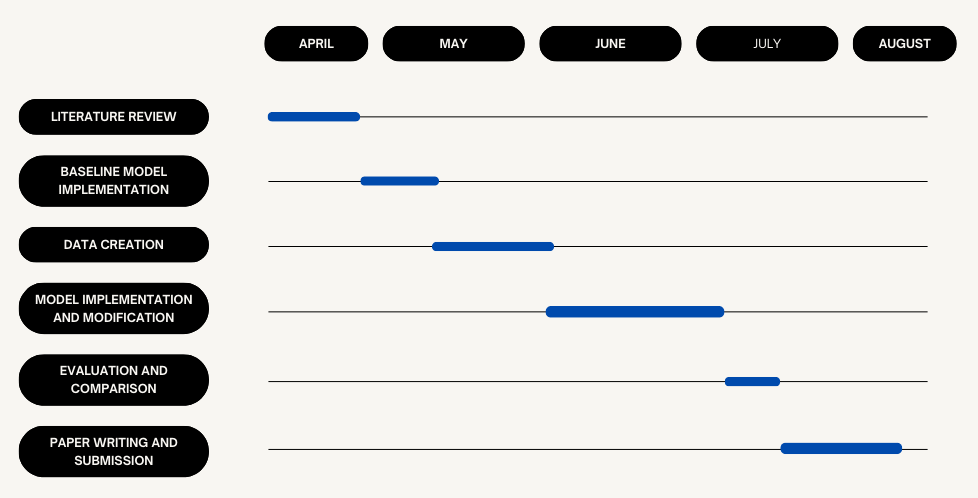
\includegraphics[width=1\textwidth]{images/gantt}
    \caption{
        Gantt diagram showing the project timeline and key milestones.
    }
    \label{fig:model}
\end{figure*}

\subsection{Outcomes and Results}\label{subsec:outcomes-and-results}
The project adapted the DCRNN model for multi-modal traffic prediction, focusing on cars and wheelchairs.
A key outcome was developing a method to derive wheelchair traffic data from existing car traffic data, addressing the
lack of wheelchair-specific datasets.
The model performed well for car traffic predictions, but its multi-modal predictions had higher error rates,
highlighting the complexity of the task.
Despite this, the project introduced valuable methodologies and laid the groundwork for future improvements in
wheelchair traffic prediction.


    \section{Research Paper}\label{sec:research-paper}
    \includepdf[pages=-]{../out/paper.pdf}

    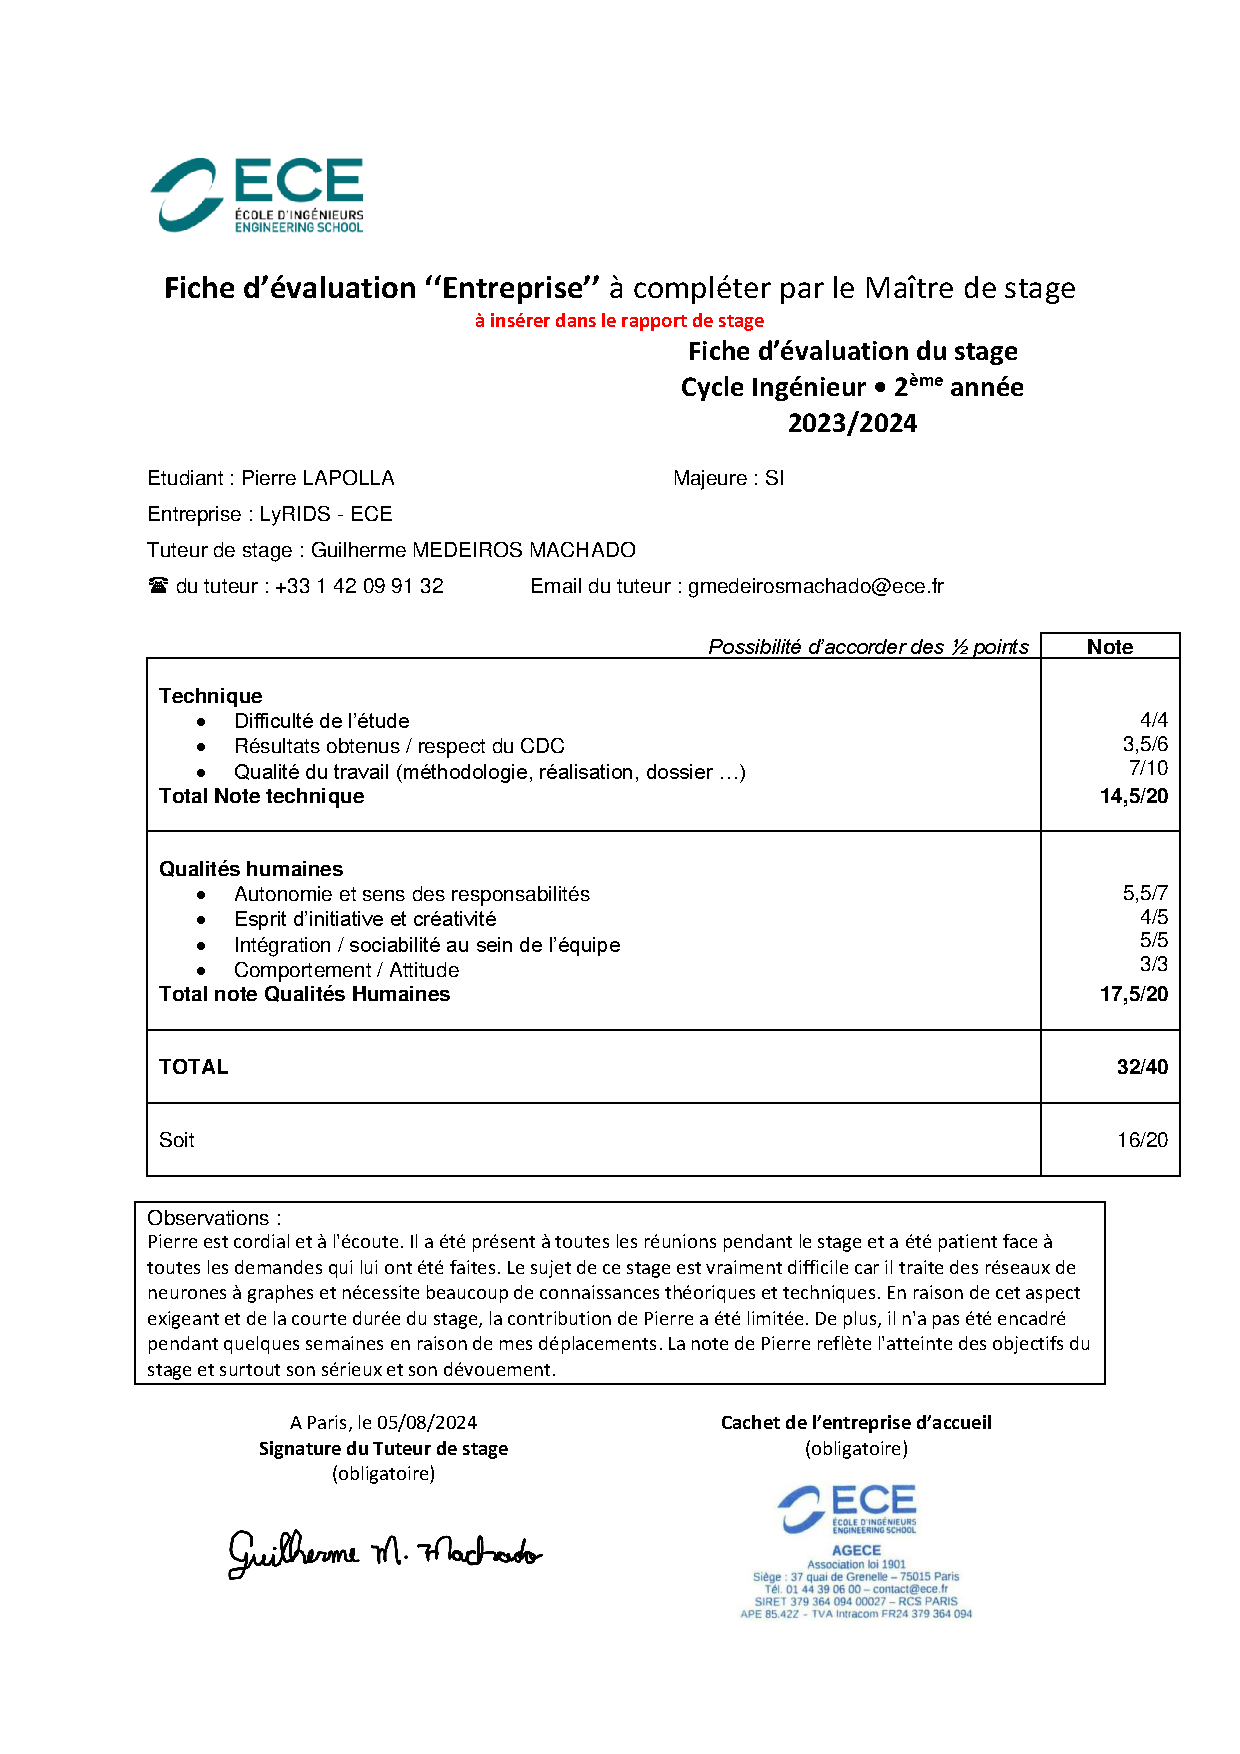
\includepdf{pdfs/evaluation.pdf}

    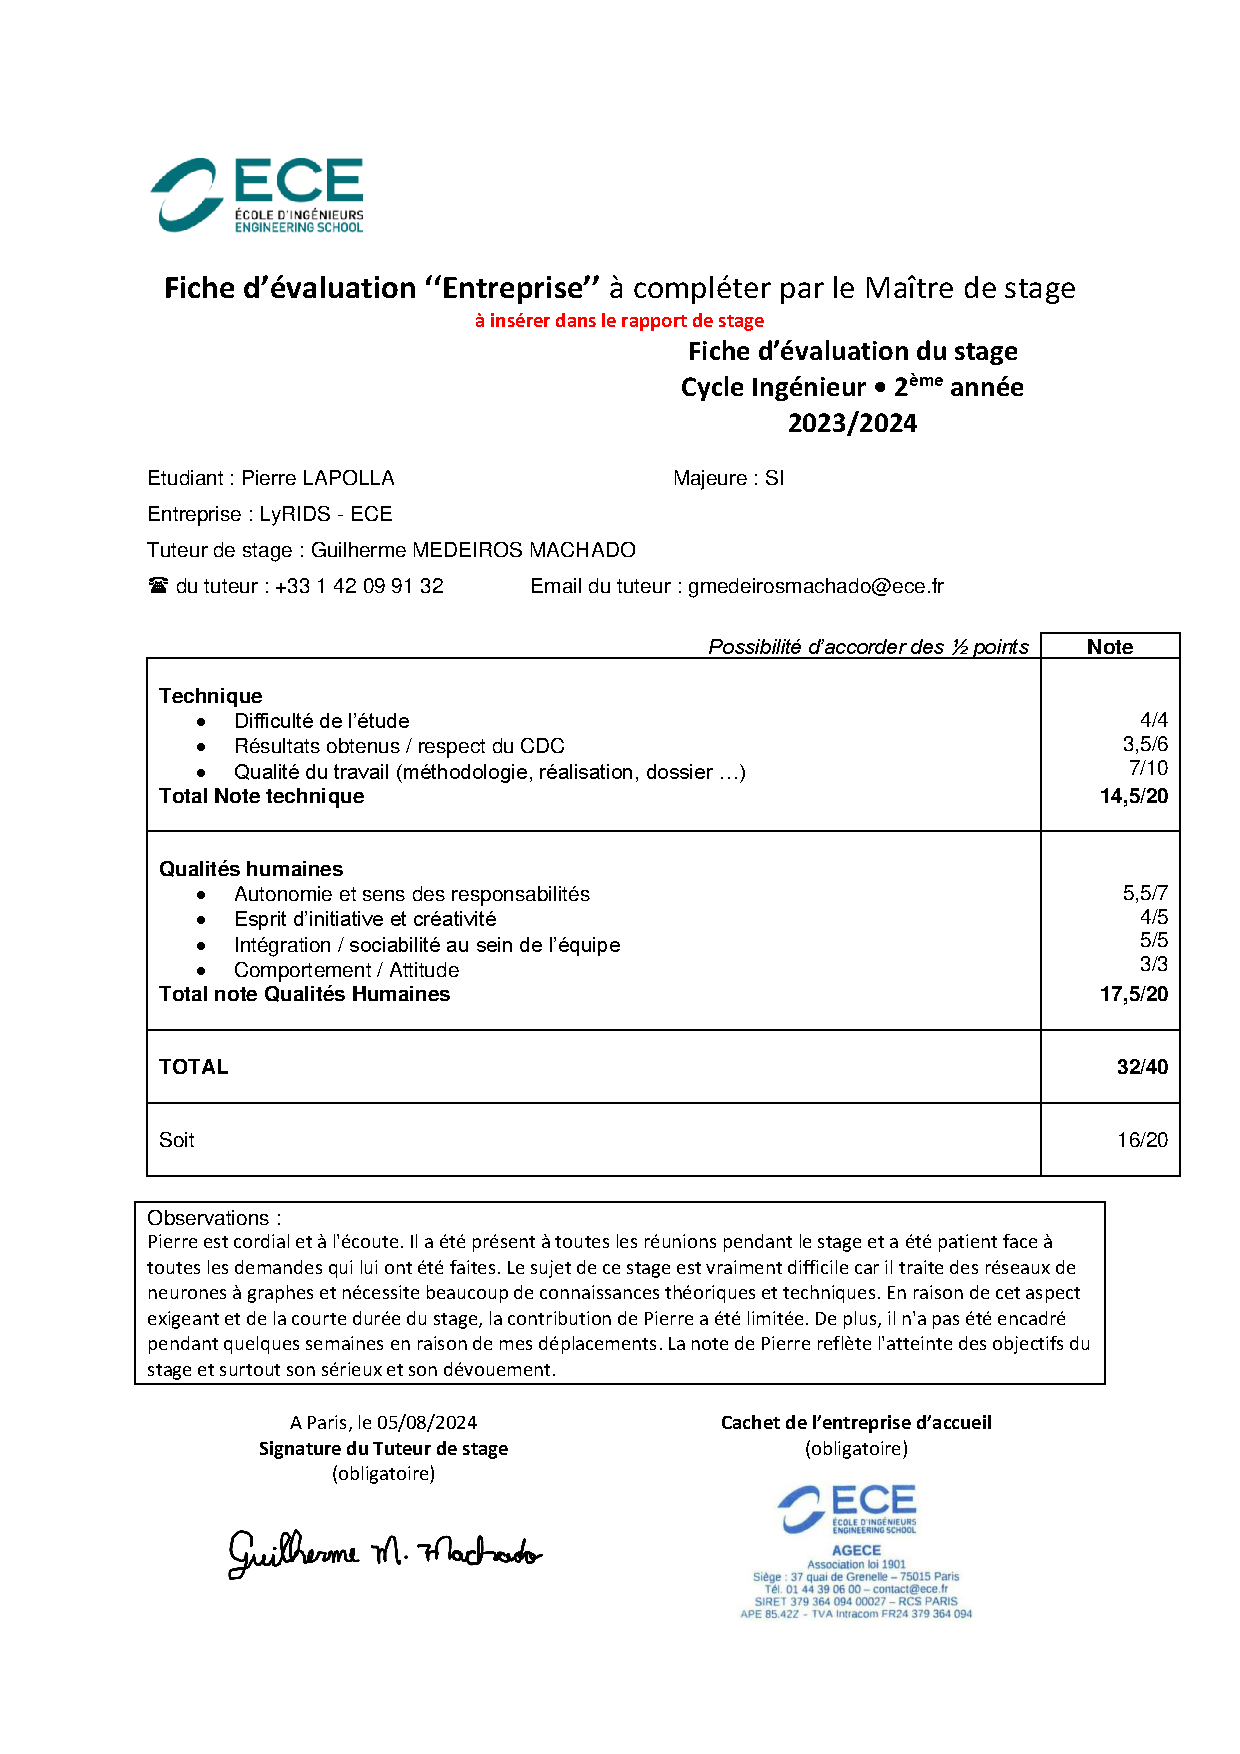
\includepdf{pdfs/notation.pdf}

\end{document}
